\centering
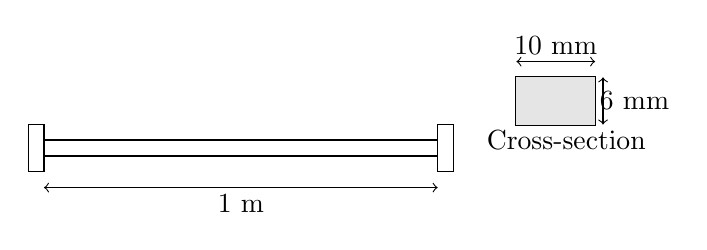
\begin{tikzpicture}
    % Draw the main beam
    \draw[thick] (0,0) -- (5,0);
    \draw[thick] (0,-0.2) -- (5,-0.2);
    
    % Add end supports
    \draw (-0.2,-0.4) rectangle (0,0.2);
    \draw (5,-0.4) rectangle (5.2,0.2);
    
    % Add dimension line and label
    \draw[<->] (0,-0.6) -- (5,-0.6);
    \node at (2.5,-0.8) {1 m};

    % Cross-section view
    \draw[thick] (6,0.2) rectangle (7,0.8);
    \fill[gray!20] (6,0.2) rectangle (7,0.8);
    
    % Cross-section labels
    \draw[<->] (7.1,0.2) -- (7.1,0.8);
    \node at (7.5,0.5) {6 mm};
    \draw[<->] (6,1) -- (7,1);
    \node at (6.5,1.2) {10 mm};
    
    % Add Cross-section text
    \node[anchor=west] at (5.5,0) {Cross-section};

\end{tikzpicture}
